\documentclass[11pt]{article}
\usepackage{amsmath}
\usepackage{hyperref}
\usepackage{bm}
\usepackage{accents} % double subscripts
\usepackage{graphicx} % Required for inserting images
\usepackage{tcolorbox}
\usepackage{tabstackengine}
\usepackage{scalerel}
\usepackage{amsfonts}
\usepackage{setspace}
\usepackage{float}
\usepackage[nocompress]{cite}
\usepackage[margin=1.6 in]{geometry}
% \author{Hao Chen\\[0.3cm]{Advisor: Prof. Manfred Sigrist}}

% \supervisors{Prof. Manfred Sigrist}

\begin{document}
\bibliographystyle{unsrt}
\newcommand{\bra}[1]{\left \langle #1 \right \rvert}
\newcommand{\ket}[1]{\left \rvert #1 \right \rangle}
\newcommand{\up}{\uparrow}
\newcommand{\down}{\downarrow}

% \maketitle
 \begin{titlepage}%
		\noindent
		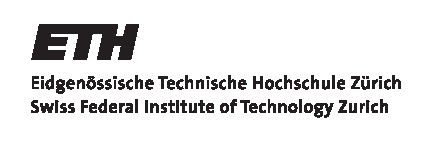
\includegraphics[viewport=8 0 185 55]{figures/eth_logo_black} \hfill
		\vspace{3cm}

		\let\footnotesize\small
		\let\footnoterule\relax
		\let \footnote \thanks


        \begin{center}
			\begin{spacing}{1.8}
			  {\huge \bfseries Non-centrosymmetric Perturbation on Superconductivity}
			\end{spacing}

            \large Semester Thesis
		\end{center}
		\vspace{0.4cm}

		\begin{center}
			\large
            Hao Chen\\
			\texttt{\small haochen1@ethz.ch}
		\end{center}%

		\vspace{0.4cm}

		\vspace{1cm}


		\vfill
		\begin{center}
			\textbf{Supervisor:} \\[2pt] Prof. Manfred Sigrist
		\end{center}

		\vspace{0.2cm}

		\begin{center}
            \today
		\end{center}
\end{titlepage}%

% \renewenvironment{abstract}
% 	{\chapter*{Abstract}}
% 	{\vfill
% 	\noindent

% 	\addcontentsline{toc}{chapter}{Abstract}
% }
\thispagestyle{plain}
\begin{flushleft}
    \vspace{0.9cm}
    \huge \textbf{Abstract}
    \vspace{0.5cm}
\end{flushleft}
We perform a perturbative calculation to investigate the effect of the
Dzyaloshinsky-Moriya interaction on a two-dimensional conventional $s$-wave superconductor.
The introduced interaction breaks the space inversion symmetry, making the system non-centrosymmetric.
By analyzing the resulting Cooper-pair wavefunction, we identify
both even-parity and odd-parity components alongside the original $s$-wave pairing,
which all belong to the $A_1$ representation of $C_{4v}$, the point group of the underlying lattice.
Surprisingly, the pairing structure remains unaffected at half-filling due to an additional
sublattice symmetry, which restricts the electrons to either form intra-sublattice pairing
or inter-sublattice pairing in real space. The pairings induced by the
Dzyaloshinsky-Moriya interaction turn out to be incompatible with the conventional $s$-wave
pairing under this symmetry, which are therefore absent at half-filling.
\newpage

\section{Introduction}
Superconductivity, a macroscopic quantum phenomenon characterized by zero resistance
below some critical temperature $T_c$,
has gathered a significant amount of attention since its discovery
over a century ago. The first theoretical breakthrough of superconductivity came from
the celebrated Bardeen-Cooper-Schrieffer (BCS) theory \cite{BCS1957}, which provided a microscopic theory
for the phenomenon and described it as a consequence of the condensation of pairing electrons (Cooper
pairs) due to the phonon-mediated attractive interactions between the electrons.
In the BCS theory, the Cooper pair has zero relative angular momentum and is a spin singlet.
The pairing structure is referred to as the conventional $s$-wave pairing.
Since then, different pairings with higher relative angular momentum have been discovered in
different materials, ranging from the superfluid phase of $^3$He \cite{Osheroff1972,Leggett1975},
the heavy fermion
compounds \cite{Stewart1984,White2015,Yoshichika2004}, to the high-$T_c$ cuprates
\cite{Dagotto1994, Tsuei2000,Anderson2004}.
In the condensed-matter jargon, any superconductor that has pairing structure different
from the conventional $s$-wave pairing is called the unconventional superconductor.

Symmetry is a powerful tool in classifying these unconventional pairing structures
\cite{Ueda1985, Volovik1985, Manfred_1991}.
In a nutshell, because the normal-to-superconducting transition is a second-order
symmetry-breaking phase transition, the order parameter of the superconducting phase furnishes
an irreducible representation of the broken symmetry, according to Landau's
phenomenological theory of the second-order phase transition \cite{Landau2013}.
Compared to the conventional pairing,
the unconventional pairing breaks additional symmetries such as the point group symmetry
besides the $U(1)$ symmetry. In that case, the order parameter in turn also belongs to
an irreducible representation of the point group symmetry. Among all symmetries,
the space inversion symmetry is a particularly important symmetry for superconductivity \cite{Anderson1984},
as it connects electrons with opposite momentums, which are the degenerated states needed to
form a Cooper pair.
For centrosymmetric systems, an immediate consequence from the symmetry perspective
is that the even and odd parity representations of the point group symmetry cannot be mixed
in the superconducting phase. In addition, because eletrons are fermionic, the constraint
implies that the Cooper pair is either spin singlet (for even-parity pairing) or
spin triplet (for odd-parity pairing) in centrosymmetric systems.

In the past decades, novel superconductors that break the inversion symmetry have been discovered
in materials such as CePt$_3$Si \cite{Bauer2004}, UIr \cite{Akazawa2004}, and
LaBiPt \cite{Goll2008}. Such non-centrosymmetric
systems allow antisymmetric spin-orbit couplings. A typical example is the Rashba spin-orbit coupling,
which has the form $\bm g(\bm k) \cdot \bm \sigma$ with $\bm g(\bm k) = \alpha(\hat{x}\sin(k_y a) -
\hat{y}\sin(k_x a))$. The coupling splits the Fermi surface and suppresses all triplet pairings but
the one with the gap $\bm d(\bm k)$ vector parallel to $\bm g(\bm k)$ \cite{Frigeri2004},
consistent with Anderson's theorem in general. Furthermore, systems without the inversion center allow an
antisymmetric exchange interaction, known as the Dzyaloshinskii–Moriya interaction.
In the following, we examine how this interaction affects the pairing structure
by doing a perturbative calculation on a toy model (see Sec.~\ref{sec:model}).
We show that a parity-mixing occurs between the spin singlet and triplet states,
in contrast to centrosymmetric superconductors. Furthermore, we find that the conventional $s$-wave
pairing is unaffected by the perturbation at half-filling, which can be understood from the additional
sublattice symmetry that arises at this special filling. We also derive a general restriction
on the pairing structures for systems with a sublattice symmetry.

\section{Microscopic model}\label{sec:model}
We start with a one-band model on a two-dimensional (2D) square lattice, defined as follows:
\begin{align}\label{eq:H}
    H &= H_0 + H_I = \underbrace{\sum_{\bm k s} \epsilon_{\bm k} c^{\dagger}_{\bm{k},s}c^{\dagger}_{\bm{k},s} - g \sum_j n_{j \uparrow}n_{j \downarrow}}_{H_0} + \underbrace{\sum_{\langle ij \rangle} \bm D_{ij} \cdot (\bm S_i \times \bm S_j)}_{H_I},
\end{align}
where the kinetic energy is $\epsilon_{\bm k} = -2t [\cos(k_x a) + \cos(k_y a)] - \mu$
and the coupling $g$ characterizes the on-site attraction. They constitute the unperturbed
Hamiltonian $H_0$. The Dzyaloshinsky-Moriya interaction $H_I$ is treated as a perturbation with $\bm D_{ij} =
D({\hat{\bm z}} \times (\bm r_i - \bm r_j))$ ($\langle ij \rangle$ denotes summing over nearest-neighbors).

The unperturbed Hamiltonian $H_0$ is symmetric under space inversion transformation
$P: P c^{(\dagger)}_{\bm r_i} P^{-1} = c^{(\dagger)}_{-\bm r_i}$ since $\epsilon_{\bm k} = \epsilon_{-\bm k}$.
The pairing structure for $H_0$ can be derived from a simple mean-field approach.
By condensing the pairing operator $c_{\bm{-k}\downarrow} c_{\bm{k} \uparrow}$ and
$c^\dagger_{\bm{k}\uparrow} c^\dagger_{\bm{-k} \downarrow}$, and diagonalizing
the resulting mean-field Hamiltonian, we arrive at
\begin{equation}\label{eq:s-wave}
    H_0 = \sum_{\bm{k}}\left\{E_{\bm{k}}{\gamma}_{\bm{k} 1}^{\dagger}
    {\gamma}_{\bm{k} 1}+E_{\bm{k}} {\gamma}_{\bm{k} 2}^{\dagger} {\gamma}_{\bm{k} 2}\right\},
\end{equation}
where additional constants are igonored, the excitation energy
$E_{\bm {k}} = \sqrt{\epsilon_{\bm {k}}^2 + \Delta^2}$,
and the Bogliubov particle $(\gamma_{\bm k}, \gamma^\dagger_{\bm k})$ is defined as
\begin{equation}
    \setstacktabbedgap{2pt}
    \left(\begin{array}{c}
    {c}_{\boldsymbol{k} \uparrow} \\
    {c}_{-\boldsymbol{k} \downarrow}^{\dagger}
    \end{array}\right)=
    \left(\begin{array}{cc}
    u_{\boldsymbol{k}} & v_{\boldsymbol{k}} \\
    -v_{\boldsymbol{k}} & u_{\boldsymbol{k}}
    \end{array}\right)
    \left(\begin{array}{c}
    {\gamma}_{\boldsymbol{k} 1} \\
    {\gamma}_{-\boldsymbol{k} 2}^{\dagger}
    \end{array}\right)
\end{equation}
with coefficients
\begin{equation}
    u_{\bm k}^2=\frac{1}{2}\left(1+\frac{\epsilon_{\bm k}}{\sqrt{\epsilon_{\bm k}^2 + \Delta^2}} \right) \quad \text {
    and } \quad v_{\bm k}^2=\frac{1}{2}\left(1-\frac{\epsilon_{\bm k}}{\sqrt{\epsilon_{\bm k}^2 + \Delta^2}}\right).
\end{equation}
The gap $\Delta$ satisfies the following self-consistent equation at $T=0$:
\begin{equation}
    \Delta = \frac{g}{2 \Omega} \sum_{\bm{k}} \frac{\Delta}{\sqrt{\epsilon_{\bm k}^2 + \Delta^2}}.
\end{equation}
In particular, the gap function $\Delta$ is a constant, corresponding to the conventional
$s$-wave pairing.
The ground state $\ket{g_0}$ of Eq.~\eqref{eq:s-wave} is the state that gets annihilated
by all $\gamma$ operators:
$\gamma_{\bm k, \sigma}\ket{g_0} = 0,\ \forall \bm{k},\sigma$.

The Dzyaloshinsky-Moriya perturbation breaks the inversion symmetry, as it changes sign under $P$:
\begin{equation}
    P \sum_{\langle ij \rangle} \bm D_{ij} \cdot (\bm S_i \times \bm S_j) P^{-1}
    = \sum_{\langle ij \rangle} \bm D_{ij} \cdot (\bm S_{-i} \times \bm S_{-j})
    = \sum_{\langle i^\prime j^\prime \rangle} -\bm D_{i^\prime j^\prime}
    \cdot (\bm S_{i^\prime} \times \bm S_{j^\prime}).
\end{equation}
Moreover, similar to the case of spin-orbit coupling, the point-group transformations of $\bm k$
and the spin transformations can no longer be treated independently due to the Dzyaloshinsky-Moriya
interaction. Specifically, $H_I$ is only invariant under the joint transformation
$g: g \bm S_{r_i} g^{-1} = R^{+}(g)\bm S_{R^-(g^{-1}) \bm r_i}$ with
$R^{\pm}$ the representation of $O(3)$ in three-dimensional space with
positive or negative inversion operation:
\begin{equation}
    \begin{aligned}
    \sum_{\langle ij \rangle} g \bm D_{ij}\cdot(\bm S_{\bm r_i} \times \bm S_{\bm r_j}) g^{-1}
    &= \sum_{\langle ij \rangle}  \bm D_{ij}\cdot(R^+(g)\bm S_{R^-(g^{-1}) \bm r_i} \times R^{+}(g)\bm
    S_{R^-(g^{-1}) \bm r_j})\\
    &= \sum_{\langle ij \rangle}  D(R^-(g)\hat{\bm z}\times(R^-(g) \bm r_i - R^-(g)\bm r_j))\cdot R^{+}(g)
    (\bm S_{\bm r_i} \times \bm S_{\bm r_j})\\
    &= \sum_{\langle ij \rangle}  D \left[R^-(g)(\hat{\bm z}\times( \bm r_i - \bm r_j))\right]\cdot
    \left [R^{+}(g) (\bm S_{\bm r_i} \times \bm S_{\bm r_j})\right]\\
    &=\sum_{\langle ij \rangle}  \bm D_{ij}\cdot(\bm S_{\bm r_i} \times \bm S_{\bm r_j}),
    \quad \forall g \in \Gamma.
    \end{aligned}
\end{equation}
Here $\Gamma$ is the point group $C_{4v}$, which is a subgroup of $O(3)$.
In the last equality, we used that both representations $R^{\pm}$ restricted
to $C_{4v}$ lead to the same representation since $P\notin C_{4v}$.
In the following, we study how this interaction alters the conventional pairing of $H_0$.

\section{Perturbative treatment}
The inversion-symmetry-breaking term written in terms of the bare electron in momentum space reads
\begin{equation}
    \begin{aligned}
    H_I &=  \frac{iD}{\Omega}\sum_{\bm k_1, \bm k_2, \bm q} \sum_{s_1 s_2 s_3 s_4} \bigg\{-\sin[q_y a] \left(\frac{\sigma^y_{s_1 s_2}}{2} \frac{\sigma^z_{s_3, s_4}}{2} - \frac{\sigma^z_{s_1 s_2}}{2} \frac{\sigma^y_{s_3, s_4}}{2}\right)\\
    &+ \sin[q_x a]
    \left(\frac{\sigma^z_{s_1 s_2}}{2} \frac{\sigma^x_{s_3, s_4}}{2}
    - \frac{\sigma^x_{s_1 s_2}}{2} \frac{\sigma^z_{s_3, s_4}}{2}\right)\bigg\}
c^\dagger_{\bm k_1 s_1} c^\dagger_{\bm{k}_2 s_3} c_{\bm {k}_2-\bm{q} s_4}
c_{\bm {k}_1 + \bm{q} s_2}.
    \end{aligned}
\end{equation}
In the following, we will take the lattice spacing $a = 1$ for convenience.
\begin{figure}[htb]
  \centering
  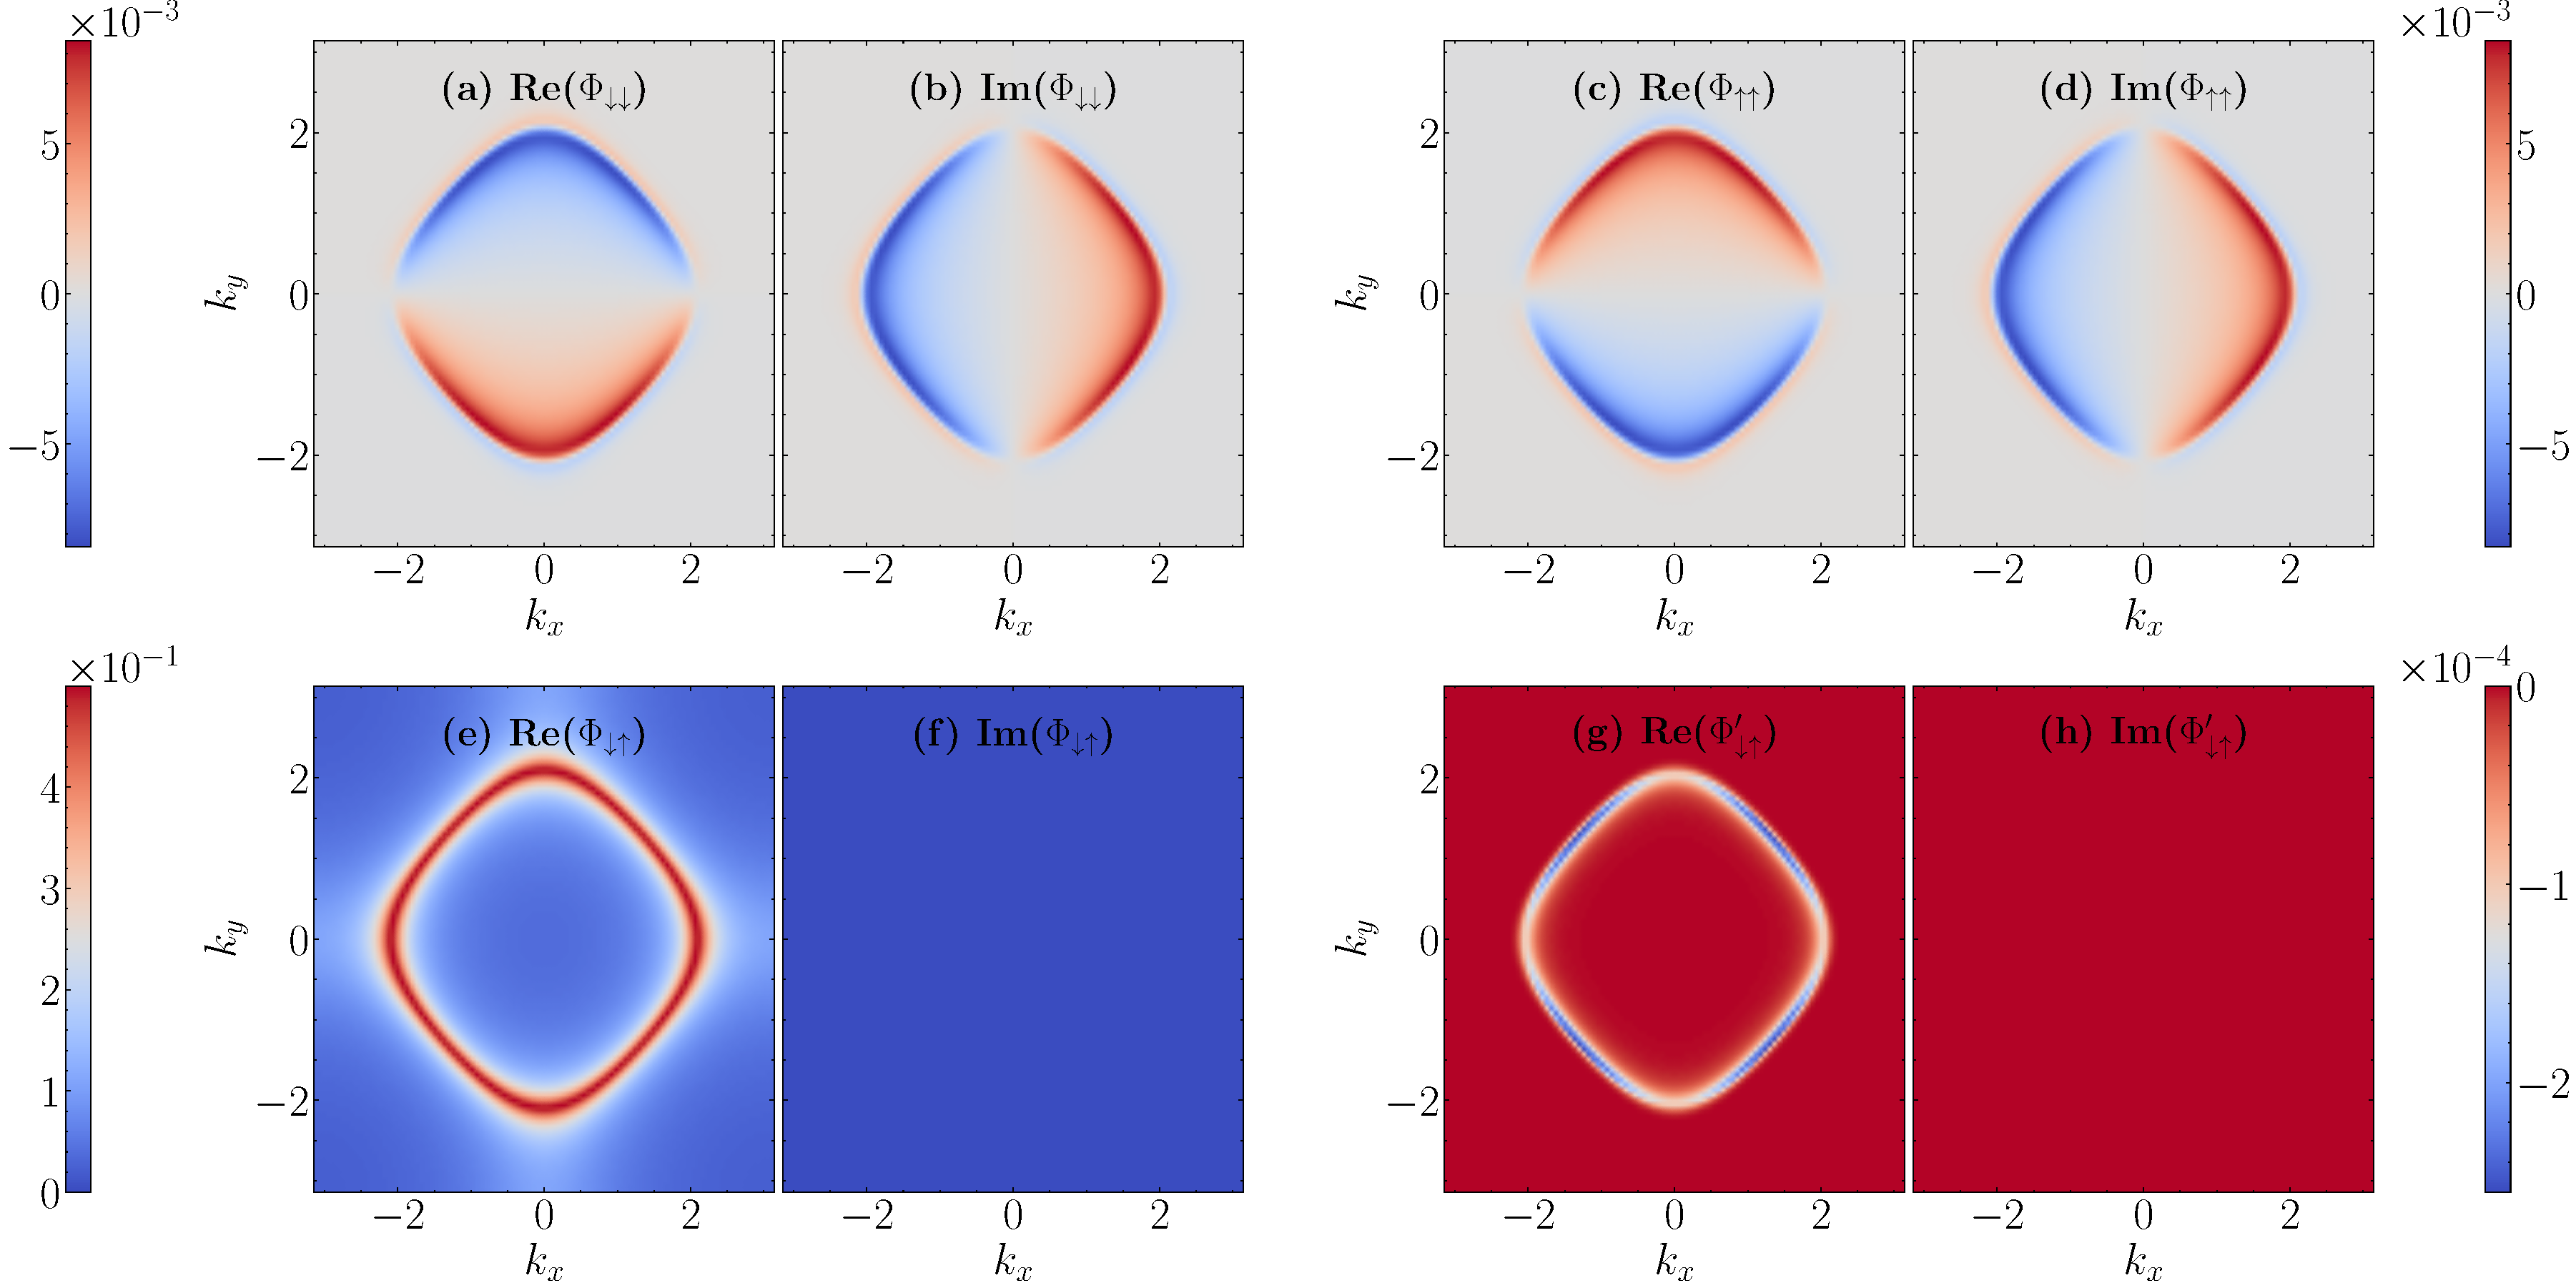
\includegraphics[width=\linewidth]{../plot/order_-1.0_2.0_0.5.pdf}
  \caption{Order parameters $\Phi_{s_1 s_2}$ at chemical potential $\mu = -1$. Other parameters are
  fixed as $(t, g, D) = (1, 2, 0.5)$. The quantity $\Phi^\prime_{\downarrow \uparrow} =
  \Phi_{\downarrow \uparrow} - \bra{g_0} c_{-\bm k \downarrow} c_{\bm k \uparrow} \ket{g_0}$
  characterizes the new singlet pairing structure due to the perturbation.}
  \label{fig:mu=-1}
\end{figure}
Analogous to the mean-field treatment, we approximate the quartic term by a sum of quadratic terms:
\begin{equation}
\begin{aligned}
    c^\dagger_{\bm k_1 s_1} c^\dagger_{\bm{k}_2 s_3} c_{\bm {k}_2-\bm{q} s_4} c_{\bm {k}_1 + \bm{q} s_2} &=
    \langle c^\dagger_{\bm k_1 s_1} c^\dagger_{\bm{k}_2 s_3} \rangle_{\scaleto{0}{3.5pt}}
    c_{\bm {k}_2-\bm{q} s_4} c_{\bm {k}_1 + \bm{q} s_2} +
    c^\dagger_{\bm k_1 s_1} c^\dagger_{\bm{k}_2 s_3}
    \langle c_{\bm {k}_2-\bm{q} s_4} c_{\bm {k}_1 + \bm{q} s_2}\rangle_{\scaleto{0}{3.5pt}} \\
    &-\langle c^\dagger_{\bm k_1 s_1} c_{\bm {k}_2-\bm{q} s_4} \rangle_{\scaleto{0}{3.5pt}}
     c^\dagger_{\bm{k}_2 s_3} c_{\bm {k}_1 + \bm{q} s_2}
    -c^\dagger_{\bm k_1 s_1} c_{\bm {k}_2-\bm{q} s_4}
     \langle c^\dagger_{\bm{k}_2 s_3} c_{\bm {k}_1 + \bm{q} s_2} \rangle_{\scaleto{0}{3.5pt}}\\
    &+\langle c^\dagger_{\bm k_1 s_1} c_{\bm {k}_1 + \bm{q} s_2}\rangle_{\scaleto{0}{3.5pt}}
     c^\dagger_{\bm{k}_2 s_3} c_{\bm {k}_2-\bm{q} s_4}
    +c^\dagger_{\bm k_1 s_1} c_{\bm {k}_1 + \bm{q} s_2}
     \langle c^\dagger_{\bm{k}_2 s_3} c_{\bm {k}_2-\bm{q} s_4} \rangle_{\scaleto{0}{3.5pt}}.
\end{aligned}
\end{equation}
To treat $H_I$ perturbatively, we evaluate the expectation values using the unperturbed ground state
$\ket{g_0}$, i.e., $\langle \cdot \rangle_{\scaleto{0}{3.5pt}} = \bra{g_0}\cdot \ket{g_0}$,
instead of determining the expectation values through self-consistent equations.
After some algebra work, we obtain the resulting Bogoliubov-de-Gennes (BdG) Hamiltonian
\begin{equation}\label{eq:BdG}
    H_{\text{BdG}} = \sum_{\bm k}\frac{1}{2}
    \begin{pmatrix}
    \gamma^\dagger_{\bm k 1} & \gamma^\dagger_{\bm k 2}& \gamma_{-\bm k 1}& \gamma_{-\bm k 2}
    \end{pmatrix}
    \left(
    \begin{array}{cccc}
    E_{\bm k} & A_{\bm k} & {B_{\bm k}} & 0 \\
    {A^*_{\bm k}} &  E_{\bm k}& 0 & -{B^*_{\bm k}} \\
    {B^*_{\bm k}} & 0 & -E_{\bm k} & -{A^*_{\bm k}} \\
    0 & -{B_{\bm k}} & -{A_{\bm k}} & -E_{\bm k} \\
    \end{array}
    \right)
    \begin{pmatrix}
    \gamma_{\bm k 1} \\
    \gamma_{\bm k 2} \\
    \gamma^\dagger_{-\bm k 1}\\
    \gamma^\dagger_{-\bm k 2}
    \end{pmatrix},
\end{equation}
where
\begin{align}
    A_{\bm k} &= \frac{D}{\Omega}\sum_{\bm {k}^{\prime}}\bigg(\sin(k_{y}^\prime - k_{y})
    +i \sin(k_{x}^\prime - k_{x})\bigg)
    u_{\bm{k}} v_{\bm{k}} u_{\bm{k}^{\prime}} v_{\bm{k}^{\prime}},\\
    B_{\bm k} &= -\frac{D}{\Omega}\sum_{\bm {k}^{\prime}}\bigg(\sin(k_{y}^\prime - k_{y})
    +i \sin(k_{x}^\prime - k_{x})\bigg)
    v_{\bm{k}}^2 u_{\bm{k}^{\prime}} v_{\bm{k}^{\prime}}.
\end{align}
The BdG Hamiltonian~\eqref{eq:BdG} is diagonalized by introducing the new particle
$(\alpha_{\bm k \lambda}, \alpha_{\bm k \lambda})$:
\begin{equation}
    \begin{pmatrix}
    \gamma_{\bm k 1} \\
    \gamma_{\bm k 2} \\
    \gamma^\dagger_{-\bm k 1}\\
    \gamma^\dagger_{-\bm k 2}
    \end{pmatrix}
    = S_{\bm k}
    \begin{pmatrix}
    \alpha_{\bm k 1} \\
    \alpha_{\bm k 2} \\
    \alpha^\dagger_{-\bm k 1}\\
    \alpha^\dagger_{-\bm k 2}
    \end{pmatrix}
\end{equation}
with $S_{\bm k}$ a unitary $4\times 4$ matrix. The diagonalized Hamiltonian is
\begin{equation}
    H_{\text{BdG}} = \sum_{\bm k} \omega_{\bm k 1} \alpha^\dagger_{\bm k 1} \alpha_{\bm k 1}
    +\omega_{\bm k 2} \alpha^\dagger_{\bm k 2} \alpha_{\bm k 2},
\end{equation}
where
\begin{align}
    \omega_{\bm k, 1} &= \sqrt{|A_{\bm k}|^2+|B_{\bm k}|^2+ E_{\bm k}^2
    -\sqrt{\left(A_{\bm k}^* B_{\bm k}+A_{\bm k} B_{\bm k}^*\right)^2 + 4 |A_{\bm k}|^2 E_{\bm k}^2 }},\\
    \omega_{\bm k, 2} &= \sqrt{|A_{\bm k}|^2+|B_{\bm k}|^2+ E_{\bm k}^2
    +\sqrt{\left(A_{\bm k}^* B_{\bm k}+A_{\bm k} B_{\bm k}^*\right)^2 + 4 |A_{\bm k}|^2 E_{\bm k}^2 }}.
\end{align}
The new ground state $\ket{g}$ is defined as the state that gets annihilated by all $\alpha_{\bm k \lambda}$.
\begin{figure}[tb]
  \centering
  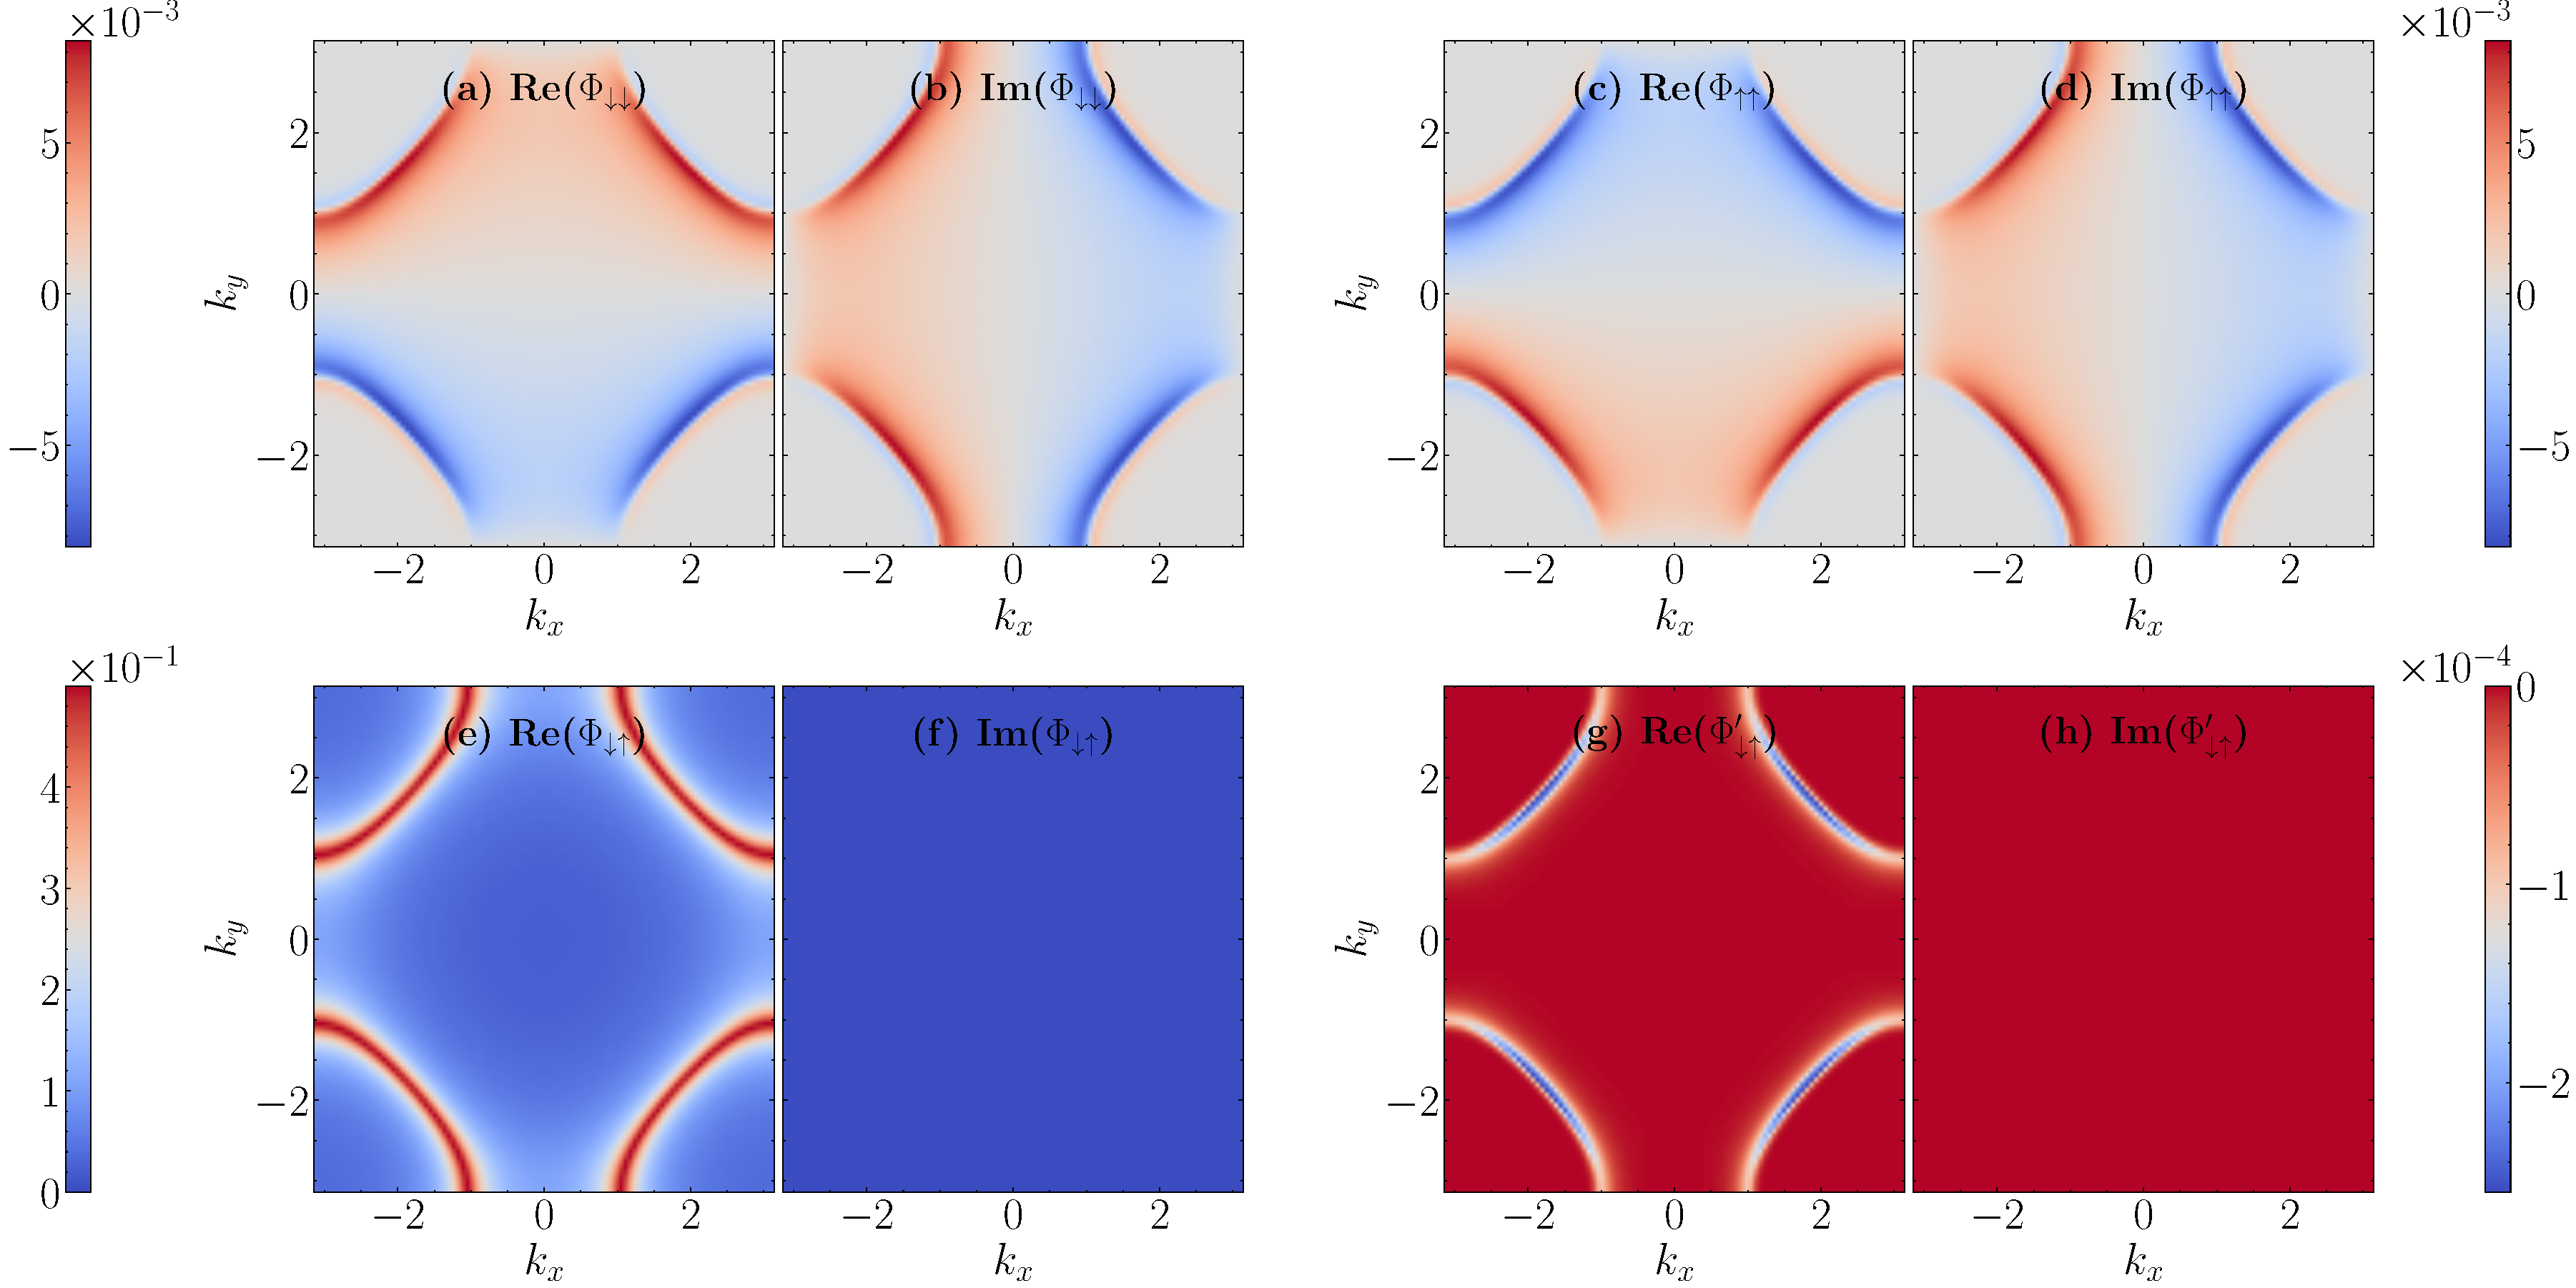
\includegraphics[width=\linewidth]{../plot/order_1.0_2.0_0.5.pdf}
  \caption{Order parameters $\Phi_{s_1 s_2}$ at chemical potential $\mu = 1$. Other parameters are
  fixed as $(t, g, D) = (1, 2, 0.5)$. The quantity $\Phi^\prime_{\downarrow \uparrow} =
  \Phi_{\downarrow \uparrow} - \bra{g_0} c_{-\bm k \downarrow} c_{\bm k \uparrow} \ket{g_0}$
  characterizes the new singlet pairing structure due to the perturbation.}
  \label{fig:mu=1}
\end{figure}

In order to study the pairing structure of the ground state $\ket{g}$, we define the order parameter
\begin{equation}\label{eq:order_parameter}
    \Phi_{s_1 s_2} = \bra{g} c_{-\bm k s_1} c_{\bm k s_2} \ket{g}.
\end{equation}
Note that we use the bare electron operators inside the bracket.
Figures.~\ref{fig:mu=-1}, \ref{fig:mu=1}, \ref{fig:mu=0} show the order parameter $\Phi_{s_1 s_2}$ for three
different choices of the chemical potential $\mu$ while fixing $t=1, g = 2, D=0.5$.
From Fig.~\ref{fig:mu=-1}(a-d) and Fig.~\ref{fig:mu=1}(a-d), we observe that odd-parity pairing emerges on top the
original even-parity pairing. Furthermore, we can get the perturbation effect on the original
s-wave singlet pairing by subtracting $\bra{g_0} c_{-\bm k \downarrow} c_{\bm k \uparrow} \ket{g_0}$
from $\Phi_{\downarrow \uparrow}$, and we denote the new quantity as $\Phi^\prime_{\downarrow \uparrow}$,
as shown in Fig.~\ref{fig:mu=-1}(g-h) and Fig.~\ref{fig:mu=1}(g-h). The pattern of $\Phi^\prime_{\downarrow \uparrow}$
implies the additional extended $s$-wave pairing of the form $\cos(k_x) + \cos(k_y)$.

Surprisingly, the non-centrosymmetric perturbation does not alter the pairing structure at half-filling
($\mu = 0$) in our calculations, as shown in Fig.~\ref{fig:mu=0}. Specifically, at $\mu = 0$,
\begin{equation}
    \begin{aligned}
        A_{\bm k} &= -\frac{u_{\bm k}v_{\bm k} D}{2}\int \frac{d^2 k^\prime}{(2\pi)^2}
        \frac{\Delta[\cos(k_y^\prime)\sin(k_y) + i\cos(k_x^\prime)\sin(k_x)]}
        {\sqrt{4t^2(\cos(k_x^\prime)+\cos(k_y^\prime))^2+\Delta^2}} = 0,\\
        B_{\bm k} &= \frac{v_{\bm k}^2 D}{2}\int \frac{d^2 k^\prime}{(2\pi)^2}
        \frac{\Delta[\cos(k_y^\prime)\sin(k_y) + i\cos(k_x^\prime)\sin(k_x)]}
        {\sqrt{4t^2(\cos(k_x^\prime)+\cos(k_y^\prime))^2+\Delta^2}} = 0.\\
    \end{aligned}
\end{equation}
Therefore, in our perturbation scheme, $H_I$ doesn't couple to $H_{0}$ at half-filling.



\begin{figure}[htb]
  \centering
  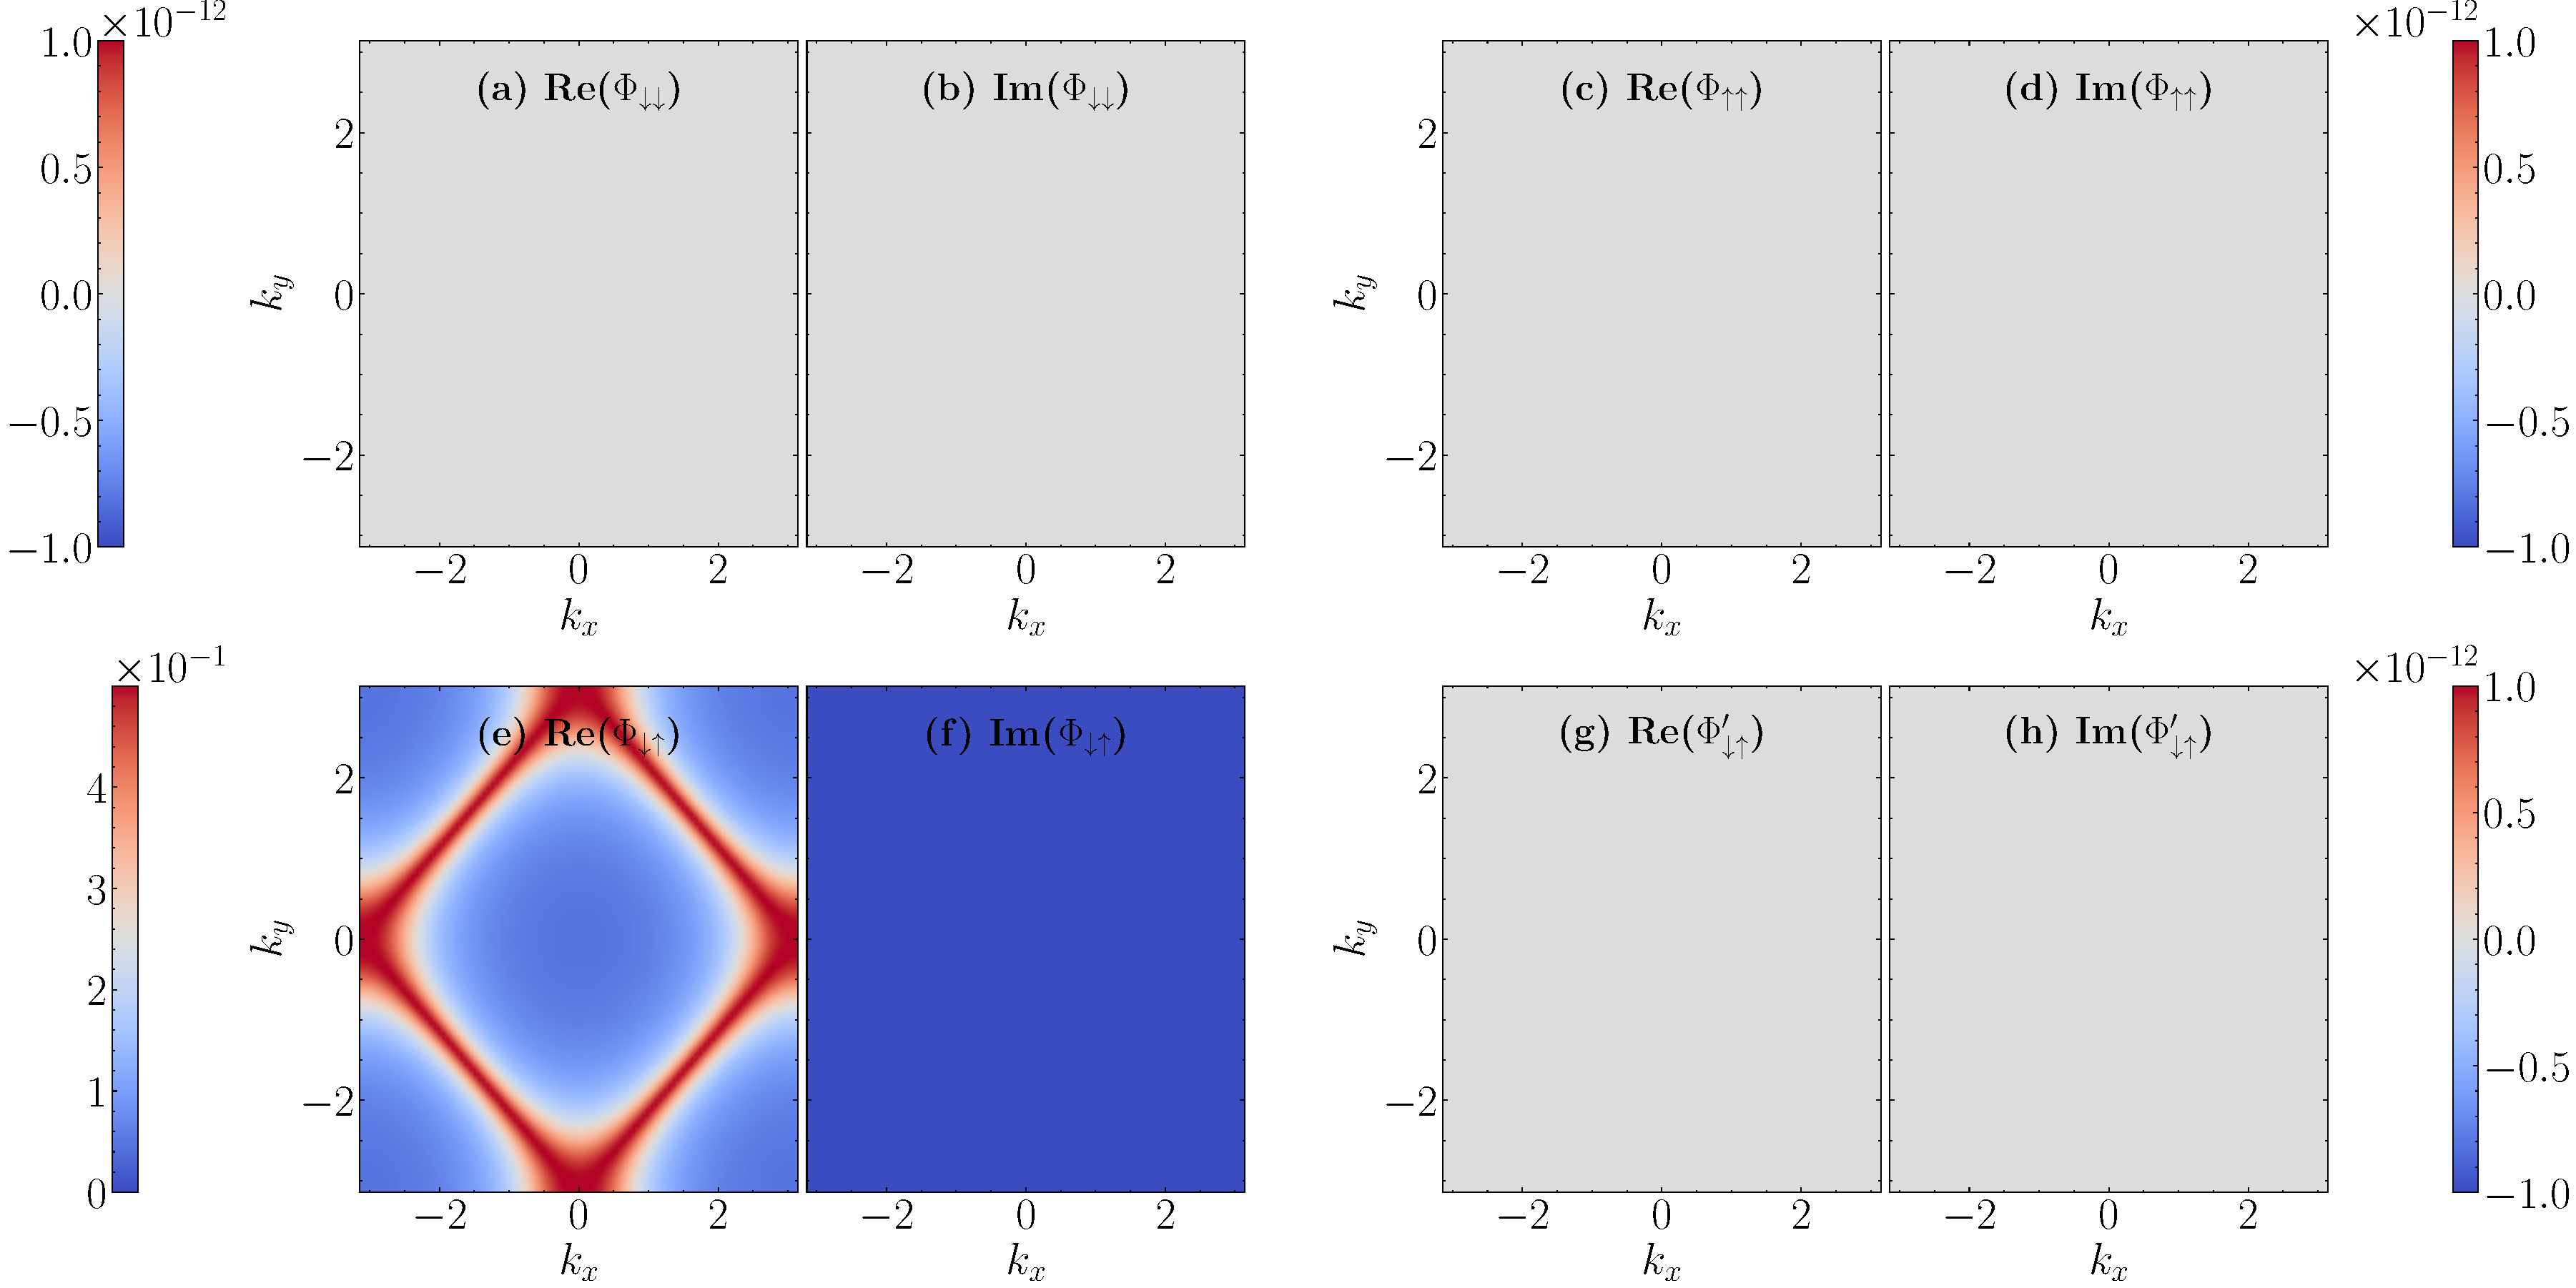
\includegraphics[width=\linewidth]{../plot/order_0.0_2.0_0.5.pdf}
  \caption{Order parameters $\Phi_{s_1 s_2}$ at chemical potential $\mu = 0$. Other parameters are
  fixed as $(t, g, D) = (1, 2, 0.5)$. The quantity $\Phi^\prime_{\downarrow \uparrow} =
  \Phi_{\downarrow \uparrow} - \bra{g_0} c_{-\bm k \downarrow} c_{\bm k \uparrow} \ket{g_0}$
  characterizes the new singlet pairing structure due to the perturbation.}
  \label{fig:mu=0}
\end{figure}

\section{Sublattice symmetry at half-filling}
We provide a symmetry argument for understanding the absence of the odd-parity pairing component at $\mu=0$,
which relies on the additional sublattice symmetry of the system at half-filling.
At half-filling ($\mu = 0$), we define the following sublattice transformation $K$:
\begin{equation}\label{eq:ph}
\begin{aligned}
    K c_{i s} K^{-1} &= c^\dagger_{i s}, \quad && i\in A\  \mathrm{sublattice},\\
    K c_{i s} K^{-1} &= -c^\dagger_{i s}, \quad && i\in B\  \mathrm{sublattice},\\
    K i K^{-1} &= -i,
\end{aligned}
\end{equation}
where we have divided the 2D square lattice into sublattices $A$ and $B$, as shown in Fig.~\ref{fig:lattice}(a),
and the last line of Eq.~\eqref{eq:ph} implies that $K$ is anti-unitarily realized in
the many-particle Fock space \cite{Ludwig2016}. The sublattice symmetry $K$ can also be
viewed as the product of the time-reversal transformation $T$ and particle-hole
transformation $\mathcal{C}$, i.e., $K = T\cdot \mathcal{C}$ with
\begin{equation}\label{eq:TC}
\begin{aligned}
    T c_{i s} T^{-1} &= (-i \sigma_y)_{s s^\prime}c_{i s^\prime}, \\
    T c_{i s} T^{-1} &= (-i \sigma_y)_{s s^\prime} c_{i s^\prime}, \\
    T i T^{-1} &= -i.
\end{aligned}
\qquad
\begin{aligned}
    \mathcal{C} c_{i s} \mathcal{C}^{-1} &= (i \sigma_y)_{s s^\prime}c^\dagger_{i s^\prime},
    \quad && i\in A\  \mathrm{sublattice},\\
    \mathcal{C} c_{i s} \mathcal{C}^{-1} &= (-i \sigma_y)_{s s^\prime} c^\dagger_{i s^\prime},
    \quad && i\in B\  \mathrm{sublattice},\\
    \mathcal{C} i \mathcal{C}^{-1} &= i.
\end{aligned}
\end{equation}

In the following, we will first show that the full-interacting Hamiltonian~\eqref{eq:H} is
invariant under $K$ at half-filling. Then the application of $K$ to the
BCS mean-field Hamiltonian is examined, from which we derive the transformation rule
for the gap function under $K$.
Based on the irreducible representations of the sublattice symmetry,
we obtain a constraint for the mixing-parity
pairing, which explains the absence of the odd-parity state at half-filling. Within this section,
we always assume $\mu=0$.
\subsection{Sublattice transformation on the full-interacting Hamiltonian}
We examine how the full Hamiltonian~\eqref{eq:H} transforms under the sublattice transformation $K$
defined above. For the hopping term, we have
\begin{align}
    K t_{ij}(c_{i s}^\dagger c_{j s} + c_{j s}^\dagger c_{i s}) K^{-1}
    &= -t_{ij}(c_{i s} c_{j s}^\dagger + c_{j s}c_{i s}^\dagger)
    = t_{ij}(c_{j s}^\dagger c_{i s} + c_{i s}^\dagger c_{j s}).
\end{align}
Therefore, the kinetic part is invariant under $K$.
For the on-site repulsive interaction, we first derive the transformation for
the particle number operator:
\begin{align}
    K n_{i s} K^{-1}&= K (c^\dagger_{is} c_{is}) K^{-1}
    = c_{i \bar{s}} c^{\dagger}_{i \bar{s}} = 1-n_{i,\bar{s}},
\end{align}
where $\bar{s} = -s$. Therefore, we have
\begin{align}
    K g n_{i \up} n_{i \down} K^{-1}&= g(1-n_{i \down})(1-n_{i\up})
    = g(1-(n_{i, \up}+n_{i\down}) + n_{i\up} n_{i\down}) = g n_{i\up} n_{i\down}
\end{align}
where we have used the half-filling condition $n_i = n_{i\up} + n_{i\down} = 1$
in the last step. Again, the on-site interaction is invariant under $K$.
For the Dzyaloshinsky-Moriya interaction, we first derive the transformations for the spin
operators:
\begin{align}
    K \vec{S}_i K^{-1}&= K (c^\dagger_{is_1} \frac{\vec{\sigma}_{s_1 s_2}}{2} c_{is_2}) K^{-1}
    =  c_{i s_1} \frac{\vec{\sigma}^*_{s_1 s_2}}{2} c^\dagger_{is_2} \nonumber\\
    &= (\delta_{s_1 s_2}-c^\dagger_{i s_2} c_{i s_1})
    (\frac{\vec{\sigma}^\dagger}{2})_{s_2 s_1}
    = c^\dagger_{i s_2} \frac{\vec{\sigma}_{s_2 s_1}}{2} c_{is_1} = \vec{S}_i,
\end{align}
from which we find that the Dzyaloshinsky-Moriya interaction $\bm D_{ij}\cdot(\bm S_i \times \bm S_j)$
is invariant under $K$.
In summary, we show that the full-interacting Hamiltonian~\eqref{eq:H} has a sublattice symmetry
at half-filling.
\subsection{Sublattice transformation on the mean-field Hamiltonian}
The mean-field Hamiltonian of Eq.~\eqref{eq:H} can be casted into the following
general BCS mean-field Hamiltonian
\begin{equation}\label{eq:MF-Hamiltonian}
    H_{\mathrm{MF}} = \sum_{\bm k, s}\epsilon_{\bm k} c^\dagger_{\bm k s} c_{\bm k s}
    + \sum_{\bm k} (\Delta_{s_1 s_2}(\bm k) c^\dagger_{\bm k, s_1}c^\dagger_{-\bm k, s_2} +
    \Delta_{s_1 s_2}^*(\bm k) c_{-\bm k, s_2} c_{\bm k, s_1}),
\end{equation}
where the gap $\Delta (\bm k) = - \Delta^T(-\bm k)$ since the eletrons are fermionic.
For non-centrosymmetric systems, the gap function is parametrized as
\begin{equation}\label{eq:gap}
    \Delta(\bm k) = i \sigma_y \psi(\bm k) + i(\bm d(\bm k)\cdot \vec{\sigma}) \sigma_y,
\end{equation}
with $\psi(\bm k) = \psi(-\bm k)$ characterizing the singlet pairing and
$\bm d (\bm k) = - \bm d(-\bm k)$ characterizing the triplet pairing.
Because the kinetic energy in $H_{\mathrm{MF}}$ is the same as that of the full Hamiltonian,
which is invariant under $K$, we now focus on how the pairing terms transform under the sublattice
transformations.

The momentum state transforms as follows under $K$:
\begin{align}
    K c_{\bm k s} K^{-1} &= \frac{1}{\sqrt{N}} \left(\sum_{i\in A} K c_{i s}
    e^{-i \bm k \cdot \bm r_i} K^{-1}
    + \sum_{i\in B} K c_{i s}e^{-i \bm k \cdot \bm r_i} K^{-1}\right) \nonumber\\
    &= \frac{1}{\sqrt{N}} (\sum_{i\in A} c_{i s}^\dagger
    e^{i \bm k \cdot \bm r_i}
    - \sum_{i\in B} c_{i s}^\dagger e^{i \bm k \cdot \bm r_i})
    =  c_{\bm k + \bm Q,s}^\dagger,
\end{align}
where $\bm Q = (\pi, \pi)$. Therefore, the pairing term transforms as
\begin{align}
    \sum_{\bm k, s_1, s_2} K \Delta_{s_1 s_2}(\bm k)  c^\dagger_{\bm k, s_1}c^\dagger_{-\bm k, s_2} K^{-1}
    &= \sum_{\bm k, s_1, s_2}\Delta_{s_1 s_2}^*(\bm k)
    c_{\bm k + \bm Q, s_1} c_{-\bm k - \bm Q, s_2} \nonumber\\
    &= \sum_{\bm k, s_1, s_2} -{\Delta}_{s_1 s_2}^*(\bm k - \bm Q)
    c_{-\bm k, s_2} c_{\bm k, s_1}.
\end{align}
By rewriting $K H_{\mathrm{MF}} K^{-1}$ in a similar form to Eq.~\eqref{eq:MF-Hamiltonian},
we get the action of $K$ on the gap function $\Delta(\bm k)$,
\begin{equation}\label{eq:action_on_gap}
    \begin{aligned}
        K: \Delta(\bm k) &\to -\Delta(\bm k - \bm Q) \\
        \implies \psi(\bm k) &\to -\psi(\bm k - \bm Q),\quad
        \bm d(\bm k) \to - d(\bm k - \bm Q).\\
    \end{aligned}
\end{equation}
In particular, the transformation $K$ acts linearly (not anti-linearly) on the gap function.
We note that the mean-field Hamiltonian may or may not break the sublattice symmetry,
depending on the specific form of the gap function $\psi(\bm k)$ and $\bm d(\bm k)$.
Nevertheless, since the sublattice symmetry
transformations form a $\mathbb{Z}_2$ group ($K^2 = 1$), the gap function is either in the trivial
representation of $\mathbb{Z}_2$ (when the sublattice symmetry is preserved) or the
non-trvial representation of $\mathbb{Z}_2$ (when the sublattice symmetry is spontaneously broken),
as detailed in the following subsection.
\begin{figure}[H]
\vspace{0.3cm}
  \centering
  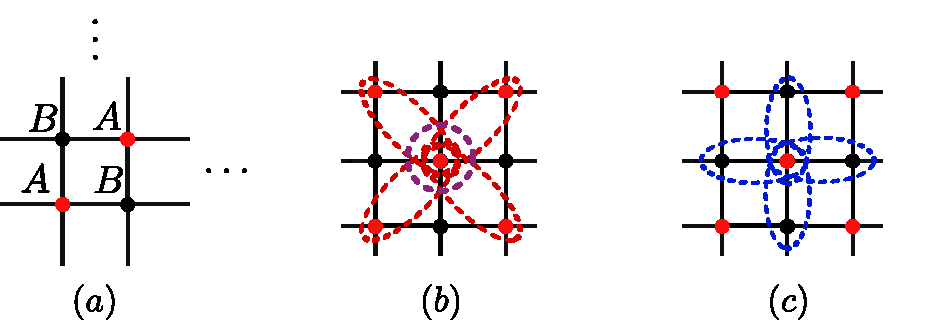
\includegraphics[width=\linewidth]{Figures/lattice.pdf}
  \caption{(a) The 2D square lattice is divided into $A$ (red) and $B$ (black) sublattices.
  (b) Intra-sublattice pairing for the sign representation $\Delta(\bm k - \bm Q) = \Delta(\bm k)$,
  as indicated by purple and red dashed lines.
  (c) Inter-sublattice pairing for the trivial representation $\Delta(\bm k - \bm Q) = -\Delta(\bm k)$,
  as indicated by blue dashed lines.}
  \label{fig:lattice}
\vspace{0.3cm}
\end{figure}

\subsection{Classification of the gap function under sublattice symmetry}
Let's first consider the simple case where the Dzyaloshinsky-Moriya interaction is ignored,
i.e., the conventional $s$-wave pairing with $\psi(\bm k) = const.$ and $\bm d(\bm k) = 0$.
In this case, the mean-field Hamiltonian $H_{\mathrm{MF}}$
is not invariant under $K$, while the full-interacting Hamiltonian (without the spin-spin coupling)
is invariant. This implies that the half-filling conventional $s$-wave pairing
breaks the $U(1)$ and sublattice symmetry simultaneously.
Hence, we can further classify the order parameter $\Delta (\bm k)$ according to the irreducible representations
of the sublattice transformations \cite{Landau2013, Manfred_1991}, i.e., a $\mathbb{Z}_2$ group.
For the conventional pairing, the order parameter belongs to the sign representation
of $\mathbb{Z}_2$, in which the non-trvial element $K \in \mathbb{Z}_2$ maps
$\psi(\bm k)$ to $-\psi(\bm k)$.

With the Dzyaloshinsky-Moriya interaction, a mixing of the even-parity and the odd-parity
states is allowed since the symmetry group changes from $D_{4h}$ to $C_{4v}$.
The mean-field Hamiltonian $H_{\mathrm{MF}}$ may or may not break the sublattice symmetry,
depending on which representation of $C_{4v}$ the order parameter $\Delta(\bm k)$ lives in. Nevertheless,
the representation should furnish an irreducible representation of $\mathbb{Z}_2$. More concretely, the gap
should satisfy either
\begin{equation}
    \begin{aligned}
    K: \Delta(\bm k) &\to -\Delta(\bm k - \bm Q) = \Delta(\bm k)
    \quad \quad \quad (\text{trivial repr. of }\mathbb{Z}_2) \\
    \implies \psi(\bm k) &\to -\psi(\bm k - \bm Q) = \psi(\bm k),\quad
    \bm d(\bm k) \to -\bm d(\bm k - \bm Q) = \bm d(\bm k),
    \end{aligned}
\end{equation}
or
\begin{equation}
    \begin{aligned}
    K: \Delta(\bm k) &\to -\Delta(\bm k - \bm Q) = -\Delta(\bm k)
    \quad \quad \quad (\text{sign repr. of }\mathbb{Z}_2) \\
    \implies \psi(\bm k) &\to -\psi(\bm k - \bm Q) = -\psi(\bm k),\quad
    \bm d(\bm k) \to -\bm d(\bm k - \bm Q) = -\bm d(\bm k).
    \end{aligned}
\end{equation}
In our model, the order parameter for the unperturbed Hamiltonian $H_0$
has the form $\psi(\bm k) = const.$ and $\bm d(\bm k) = 0$,
which furnishes a sign representation for the sublattice transformation.
When the perturbation is weak, we expect that the gap function $\Delta(\bm k)$
remains in the sign representation by continuity.
Therefore, we obtain that $\psi(\bm k)$ and $\bm d(\bm k)$ should satisfy
$\psi(\bm k) = \psi(\bm k - \bm Q)$ and $\bm d(\bm k - \bm Q) = \bm d(\bm k)$, respectively.
On the other hand, the Dzyaloshinsky-Moriya perturbation can be rewritten as
\begin{equation}
    \begin{aligned}
    H_I &\approx \frac{1}{2} \sum_{\bm k \bm k^\prime} \sum_{s_1 s_2 s_1^\prime s_2^\prime}
    \sum_{\nu} \frac{D}{4}
    \Bigg ([\phi_s(\bm k) g_s^\nu(\bm k^\prime) - \phi_d(\bm k) g_d^{\nu}(\bm k^\prime)]
    (i \sigma^y)_{s_1 s_2} (i \sigma^{\nu}\sigma^y)^\dagger_{s_2^\prime s_1^\prime}\\
        &+[\phi_s(\bm k^\prime) g_s^\nu(\bm k) - \phi_d(\bm k^\prime) g_d^{\nu}(\bm k)]
    (i \sigma^{\nu}\sigma^y)_{s_1 s_2} (i \sigma^y)^\dagger_{s_2^\prime s_1^\prime}
    \Bigg) c^\dagger_{\bm k s_1}
    c^\dagger_{-\bm k s_2} c_{-\bm k^\prime s_2^\prime} c_{\bm k^\prime s_1^\prime},
    \end{aligned}
\end{equation}
where we restrict to zero-momentum Cooper-pair scatterings. The basis functions
$(\phi_s(\bm k)$, $\bm g_s(\bm k))$ and $(\phi_d(\bm k), \bm g_d(\bm k))$ live in the
$A_1$ and $B_1$ irreducible representations of $C_{4v}$, respectively:
\begin{align}
A_1 \text{ irrep of } C_{4v}:
\phi_s(\bm k) &= \cos(k_x) + \cos(k_y),
\quad \bm g_s(\bm k) = \sin(k_y)\hat{\bm x} - \sin(k_x) \hat{\bm y};\\
B_1 \text{ irrep of } C_{4v}:
\phi_d(\bm k) &= \cos(k_x) - \cos(k_y),
\quad \bm g_d(\bm k) = \sin(k_y)\hat{\bm x} + \sin(k_x) \hat{\bm y}.
\end{align}
Because the unperturbed gap function $\psi(\bm k) = const.$ belongs to
the $A_1$ representation of $C_{4v}$, the possible pairing channels induced
by the Dzyaloshinsky-Moriya perturbation
are $\psi^{\text{(ind)}}(\bm k) \propto \cos(k_x) + \cos(k_y)$
and $\bm d^{\text{(ind)}}(\bm k) \propto \sin k_y \hat{\bm x} - \sin k_x \hat{\bm y}$,
which are incompatible with
the constraint $\psi(\bm k) = \psi(\bm k - \bm Q)$ and $\bm d(\bm k - \bm Q) = \bm d(\bm k)$.
Consequently, at half-filling there is no induced parity-mixing pairing.

More generally, the sublattice symmetry at half-filling restricts the electrons to either form
intra-sublattice pairing or inter-sublattice pairing in real space. To show this, we introduce
the pairing wavefunction in real space
\begin{equation}\label{eq:pairing_real}
\Phi_{s s^\prime}(\bm r_i - \bm r_j) = \langle c_{i s} c_{j s^\prime} \rangle
= \frac{1}{\Omega} \sum_{\bm k} \langle c_{\bm k s} c_{-\bm k s^\prime} \rangle
e^{i\bm k \cdot(\bm r_i - \bm r_j)}.
\end{equation}
Since $\langle c_{\bm k s} c_{-\bm k s^\prime} \rangle$ has the same symmetry as the gap $\Delta(\bm k)$,
the two representations of $\mathbb{Z}_2$ lead to two different pairing patterns:
\begin{equation}
\begin{aligned}
    \Delta(\bm k) = \Delta(\bm k - \bm Q)&\implies
\Phi_{s s^\prime}(\bm r_i - \bm r_j) =
\frac{1}{\Omega} \sum_{\bm k} \langle c_{\bm k s} c_{-\bm k s^\prime} \rangle
e^{i\bm k \cdot(\bm r_i - \bm r_j)}\\
&= \frac{1}{\Omega} \sum_{\bm k} \langle c_{\bm k s} c_{-\bm k s^\prime} \rangle
e^{i(\bm k- \bm Q)\cdot(\bm r_i - \bm r_j)} = 0,\  \text{ for } i\in A, j \in B,
\end{aligned}
\end{equation}
corresponding to the intra-sublattice pairing, and
\begin{equation}
\begin{aligned}
    \Delta(\bm k) = -\Delta&(\bm k - \bm Q)\implies
\Phi_{s s^\prime}(\bm r_i - \bm r_j) =
\frac{1}{\Omega} \sum_{\bm k} \langle c_{\bm k s} c_{-\bm k s^\prime} \rangle
e^{i\bm k \cdot(\bm r_i - \bm r_j)}\\
&= -\frac{1}{\Omega} \sum_{\bm k} \langle c_{\bm k s} c_{-\bm k s^\prime} \rangle
e^{i(\bm k- \bm Q)\cdot(\bm r_i - \bm r_j)} = 0,\  \text{ for } i, j\in A \text{ or } i, j \in B,
\end{aligned}
\end{equation}
corresponding to the inter-sublattice pairing, as illustrated in Fig.~\ref{fig:lattice}(b-c).
Combined with the irreducible representations of the point group, the possible forms of the
pairing wavefunction at half-filling is quite limited.
\section{Conclusion}
In this work, we explore the perturbative effect of the Dzyaloshinsky-Moriya interaction $H_I$
on a conventional $s$-wave superconductor with on-site interactions, situated on a 2D square lattice.
The additional interaction $H_I$ breaks the inversion symmetry of the system and reduces the
symmetry group from $D_{4h}$ to $C_{4v}$. Physically, it explicitly introduces a coupling between
the even-parity pairing channel and the odd-parity pairing channel.

Using a perturbative approach, we find that,
for generic chemical potential $\mu \neq 0$, the Cooper pair wavefunction has both the even-parity
component $\psi(\bm k) \propto \cos(k_x) + \cos(k_y)$ and the odd-parity component
$\bm d(\bm k) \propto \sin(k_y) \hat{\bm x} - \sin(k_x) \hat{\bm y}$, in addition to the original
conventional $s$-wave pairing $\psi(\bm k) = const$. The result
is consistent with the group-theoretical perspective, as both the
induced pairings and original pairing fall into the $A_1$ representation of $C_{4v}$.

Besides, we observe that the pairing structure is unaffected by the perturbation at $\mu = 0$,
which can be explained by the presence of an extra sublattice symmetry at half-filling.
We demonstrate that the full-interacting Hamiltonian at half-filling is symmetric under
the sublattice transformation $K$, defined in
Eq.~\eqref{eq:ph}. In the superconducting phase, the system may or may not break this
additional symmetry spontaneously, in conjunction with $U(1)$ and the point group $C_{4v}$.
Consequently, this allows us to
further classify the order parameter $\Delta$ in the irreducible representation of $\mathbb{Z}_2$.
We find that the induced pairing channels by $H_I$ are incompatible with the conventional
pairing channel under the sublattice symmetry, clarifying the absence of parity-mixing pairing.
In real space, the sublattice symmetry $K$ can be understood as requiring the electrons to
form either intra-sublattice pairing or inter-sublattice pairing.

\bibliography{refs} % Entries are in the refs.bib file
\end{document}


